% !Mode:: "TeX:UTF-8"
%!TEX program  = xelatex

\documentclass[bwprint]{cumcmthesis}
\usepackage{colortbl}
\usepackage{float}
\usepackage{cite}
\usepackage{url}

\usepackage{animate}
\usepackage{fontspec}
\newfontfamily\courier{Courier New}

\usepackage{graphicx} %use graph format  
\usepackage{subfig}  

\usepackage{listings}
\usepackage{xcolor}
\usepackage{color}
\usepackage{framed}

\definecolor{shadecolor}{rgb}{0.92,0.92,0.92}

\lstset{breaklines}
\lstset{
	numbers=left, 
	numberstyle= \tiny, 
	keywordstyle= \color{ blue!70},
	commentstyle= \color{red!50!green!50!blue!50}, 
	frame=shadowbox, % 阴影效果
	rulesepcolor= \color{ red!20!green!20!blue!20} ,
	escapeinside=``, % 英文分号中可写入中文
	xleftmargin=2em,xrightmargin=2em, aboveskip=1em,
	framexleftmargin=2em,
	basicstyle = \courier
} 


\begin{document}
\begin{center}
	{\shortstack[c]{
			\huge{\textbf{神经网络与深度学习}} \vspace{2mm}\\
			第36组\quad 王晨曦\ 汤佳俊\ 黄永锡}}
\end{center}

\begin{abstract}
	
	神经网络是一种自动化拟合函数的模型,它从人脑的生理结构出发来研究人的智能行为,模拟人脑信息处理的功能,具有并行处理的能力、自学习能力和推理能力,是根植于神经科学、数学、物理学、计算机科学及工程等科学的一种技术。现在使用的神经网络大多属于BP神经网络。
	
	BP神经网络包含了输入层、输出层和隐含层,隐含层在输入层和输出层之间,数量不固定。神经层实质上为向量化的数据或特征,连接相邻两个神经层的矩阵参数称为权重,神经网络的前向传播,多半为激活函数和矩阵乘法的组合。根据网络输出,我们可以定义损失函数,用于评估网络的拟合程度。在反向传播过程中,利用梯度下降算法可以优化网络参数,减小损失函数。
	
	神经网络的训练过程对最终结果的影响尤为重要,在数据预处理、选择训练参数等方面切不可大意。
	
	然而,浅层神经网络对函数的拟合能力还是较弱,近些年人们开始大力开发深度网络的潜能,提出了深度学习的概念。现在的深度学习技术中,最具代表性的就是卷积神经网络。
	
	与一般神经网络不同,在卷积神经网络中,输入的数据往往为类似于图片的三维数据。卷积神经网络最主要的三个结构分别为卷积层、池化层和全连接层,卷积层在抽取数据特征上有很大作用,池化层在降低数据长宽尺寸的基础上将局部信息逐渐全局化,全连接层则多用于数据尺寸和大小的线性变换。
	
	深度网络中很容易出现过拟合现象,通过一些技巧可以缓解,但如果数据量不足以支撑复杂的网络,这个问题就无法解决。深度学习向人们展示了延伸网络的巨大优势,但要指出的是,网络并不是越深越好。归根究底,深度学习只是一种工具,算法才是核心。
	
	报告中给出了两个例题,第一题为用神经网络预测公路运量,第二题为在CIFAR-10数据集上训练简单的卷积神经网络模型,相关代码和详细注释存放在代码文件夹下。
    
    报告的最后一章分析了神经网络在美赛中的具体应用,解法均来自当年的O奖试卷。通过分析我们可以看出,神经网络一般被作为求解工具来使用,不适合作为主干模型。此外,将神经网络与其他模型结合起来,充分利用各项优势,是一种不错的选择。
	
	\begin{keywords}
		\quad 神经网络\quad 损失函数\quad 梯度下降\quad 深度学习\quad 卷积神经网络\quad 过拟合
	\end{keywords}
	
\end{abstract}

\section{神经网络}

\subsection{神经网络简介}
人工神经网络(Artificial Neural Network),又称神经网络(Neural Network),最早提出于20世纪40年代,自从80年代开始被推广应用\cite{李硕2011科技传播},是由大量的处理单元(亦称为神经元)广泛互联而成的网络。它从人脑的生理结构出发来研究人的智能行为,模拟人脑信息处理的功能,是根植于神经科学、数学、物理学、计算机科学及工程等科学的一种技术。图\ref{NeuronAndNN}是人脑神经与神经网络的简单比较。

\begin{figure}[!h]
	\centering=
	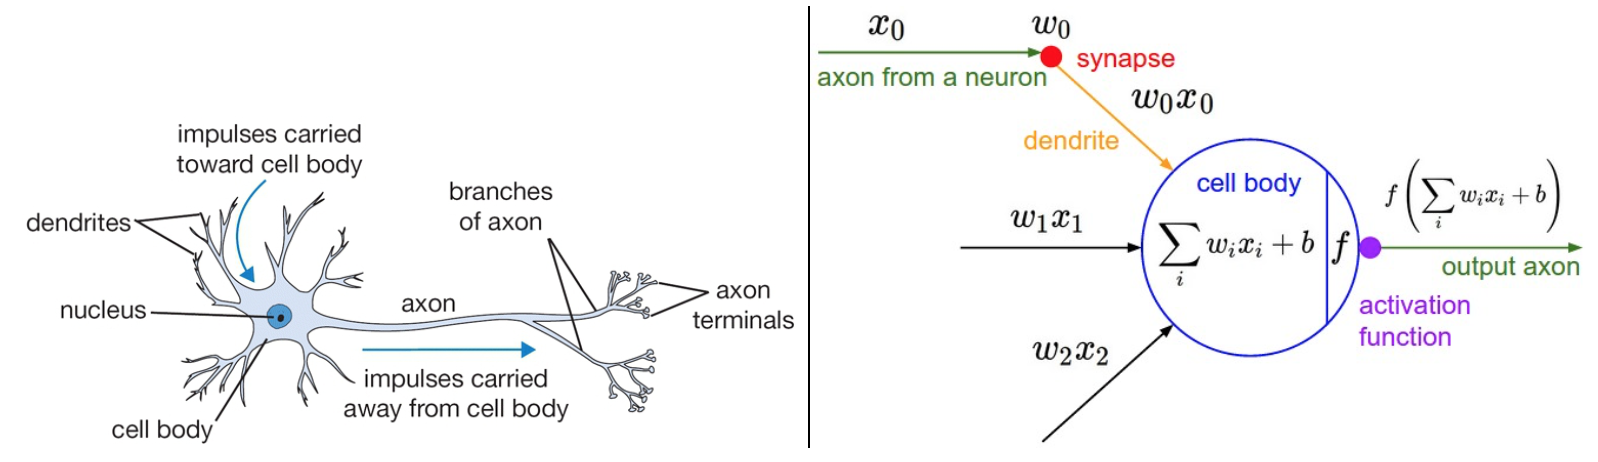
\includegraphics[width=\textwidth]{NeuronAndNN.png}
	\caption{人脑神经与神经网络对比\cite{cs231n}}
	\label{NeuronAndNN}
\end{figure}


神经网络最大的特点是其宛如一个黑箱,提供合适的数据,它会输出我们需要的结果。神经网络具有并行处理的能力、自学习能力和推理能力,主要用于数据建模、预测、模式识别和函数优化等\cite{MATLAB}。


神经网络中最常用的是BP神经网络,接下来的介绍中用到的神经网络均为BP神经网络。

\subsection{BP神经网络的基本结构}

\subsubsection{基本组成}
\begin{figure}[!h]
	\centering
	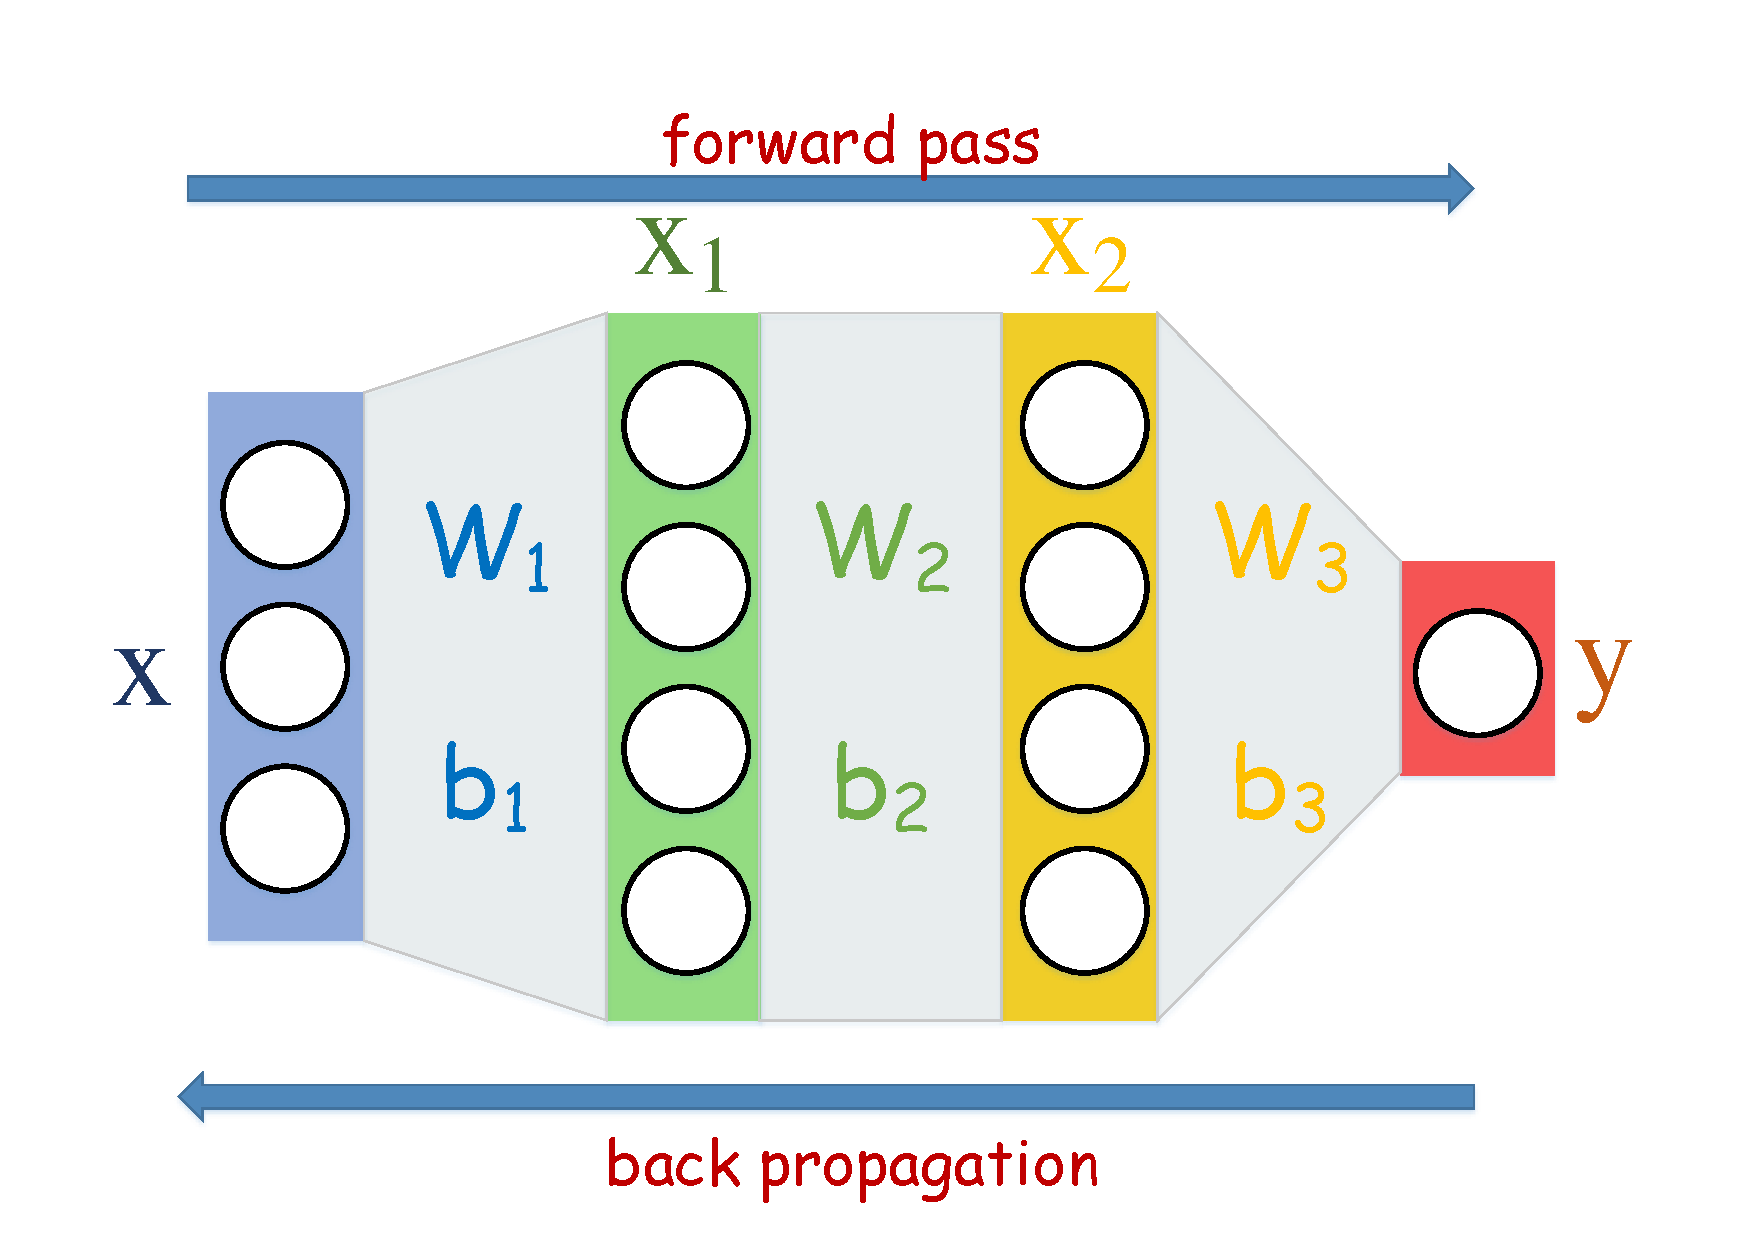
\includegraphics[width=0.8\textwidth]{NNStruct.pdf}
	\caption{BP神经网络的前向传播与反向传播}
	\label{NNStruct}
\end{figure}
一个神经网络起码要包含输入层(Input Layer)、输出层(Output Layer)和隐含层(Hidden Layer),它们实际上是已经预设好尺寸的向量,向量中的单个元素称为神经元(Neuron)。其中隐含层是指位于输入层和输出层之间的神经层,一个神经网络中可以有多层隐含层。在同一层中,神经元之间互相没有联系,而在相邻的两层间实现了全连接,连接他们的是网络的权值$W$,其数学表示为包含大量参数的矩阵。

如图\ref{NNStruct}所示,令输入数据为具有$n$个维度的列向量,输入层和第一个隐含层之间的参数为$W_1$和$b_1$,其中$W_1$是一个大小为$n\times m$的二维矩阵,$b_1$为$m$维列向量,也即

\[
x = \left[
\begin{matrix}
a_1\\ a_2\\ \vdots\\ a_n
\end{matrix}
\right],
W_1 = \left[
\begin{matrix}
p_{11} & p_{12} & \cdots & p_{1m}\\
p_{21} & p_{22} & \cdots & p_{2m}\\
\vdots & \vdots & \ddots & \vdots\\
p_{n1} & p_{n2} & \cdots & p_{nm}
\end{matrix}
\right],
b_1 = \left[
\begin{matrix}
q_1\\ q_2\\ \vdots\\ q_m
\end{matrix}
\right]
\]

则隐含层的输出为
\[x_1 = W_1\times x + b_1\]
$x_1$是一个$m$维向量。同理可得:
\[
\begin{split}
x_2 &= W_2\times x_1 + b_2\\
y &= W_3\times x_2 + b_3
\end{split}
\]

该公式是神经网络前向传播中最为关键的公式,我们通过一次次矩阵乘法不断变换输入向量的维度,最终得到拟合的结果。

\subsubsection{激活函数} 让我们联想一下生物体中神经元传递信号的方式,当突触内外电压达到一定的阈值时,神经元才会发出电信号向前传播,类比这个原理,我们在神经网络中定义了激活函数。

激活函数常用于每一次乘法操作之后,通常为非线性函数,在这里我们统一用$g(x)$来表示,将激活函数加入神经网络后,向量的变换公式变成如下形式:
\[
\begin{split}
&x_1 = g(W_1 x + b_1)\\
&x_2 = g(W_2 x_1 + b_2)\\
&y = g(W_3 x_2 + b_3)
\end{split}
\]

常用的激活函数如下:

\textbf{Sigmoid函数}

Sigmoid函数是一个在生物学中常见的S型的函数,也称为S型生长曲线。数学公式是
\[\sigma (x) = \frac{1}{1 + e^{-x}}\]

在信息科学中,由于其单增以及反函数单增等性质,Sigmoid函数常被用作神经网络的阈值函数,将变量映射到0和1之间。

在历史上,Sigmoid函数很常用,这是因为它对于神经元的激活频率有良好的解释:从完全不激活到在求和后的最大频率处的完全饱和的激活\cite{cs231n}。

\textbf{tanh函数}

tanh函数与Sigmoid函数并无本质上的差异,只是将空间中的点做了平移变换和伸缩变换,将值域从$[0,1]$映射到$[-1,1]$。其表达式为:
\[\tanh (x) = 2\sigma (2x) - 1 = \frac{1-e^{-2x}}{1+e^{-2x}}\]

和Sigmoid神经元一样,它也存在饱和问题,但是和Sigmoid神经元不同的是,它的输出是零中心的。因此,在实际操作中,tanh函数比Sigmoid函数更受欢迎。

\textbf{ReLU函数}

ReLU的全称为Rectified Linear Units,是一种十分简单直观的函数,其表达式如下:
\[\mathrm{ReLU}(x) = \max(0,x)\]

近年来ReLU函数已经成为最流行的激活函数,它有如下特点:(1)相较于Sigmoid和tanh函数,ReLU函数对于随机梯度下降的收敛有巨大的加速作用(Krizhevsky等指出有6倍之多\cite{Alex2012NIPS};(2)Sigmoid和tanh函数含有指数运算等耗费计算资源的操作,而ReLU可以简单地通过对一个矩阵进行阈值计算得到,大大提升了速度\cite{cs231n}。

图\ref{ActivationFunction}展示了三种激活函数的图像。
\begin{figure}[!h]
	\centering
	\begin{tabular}{c|c|c} 
		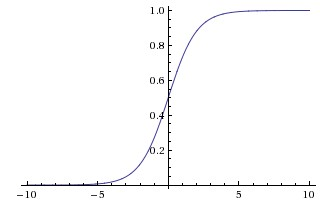
\includegraphics[height=0.14\textheight]{sigmoid.jpg} &
		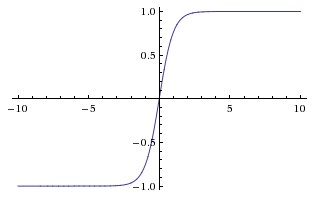
\includegraphics[height=0.14\textheight]{tanh.jpg} &
		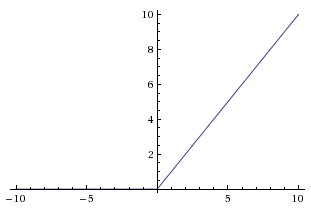
\includegraphics[height=0.14\textheight]{relu.jpg} \\
		Sigmoid函数 & tanh函数 & ReLU函数\\
	\end{tabular}
	\caption{常见激活函数\cite{cs231n}}
	\label{ActivationFunction}
\end{figure}

激活函数是神经网络中重要的组件,也是必不可少的内容,这并不是因为其在仿生学上的意义。不妨设想一下,在含有多个隐含层的网络中,如果没有激活函数,相邻层之间只有矩阵的线性变换,不难推出,经历多次线性变换与经历一次线性变换并无本质上的差别。如果我们拟合的函数是线性函数尚且没问题,但在真实情况下我们需要拟合的更多是非线性函数,而且往往是人难以直接定义的复杂函数关系。

回过头来看看激活函数,它们多为非线性函数,每经过一次激活函数就相当于数据经历了一次非线性操作,这对于函数拟合本身有很大的帮助,因此,在网络中添加激活函数是必要的。实践中也证明其在函数拟合上的作用相当之大。

\subsubsection{损失函数}
神经网络最大的特点在于其能够自主学习并优化参数,使得输出的结果不断逼近真实的函数值。为了知道如何调整参数,我们首先需要知道网络的预测值与真实值有多大的差距,为此,我们需要一种计算理想和现实间的距离的函数,也即损失函数(Loss Function)。损失函数是BP神经网络的最后一个部分,它代表了预测值与真实值之间的差异,可以想象,如果网络参数足够好的话,损失函数的值应该会很小。

在一般的函数拟合中,我们常常用均方差函数(MSE):
\[L(y, \hat{y}) =  \frac{1}{n}\sum\limits^{n}_{i=1}(y_i - \hat{y_i})^2\]
其中$y$和$\hat{y}$分别为网络的多组预测值和实际值,$i$表示某对数据对应的序号。

在较为复杂的分类问题中,我们往往还会用到Logistic回归:
\[a_i = \sigma(y_i)\]
\[L_i(a_i, \hat{y_i}) = -[\hat{y_i}\log a_i + (1-\hat{y_i})\log(1-a_i)]\]
最终得到
\[L = \frac{1}{n}\sum\limits^{n}_{i=1}L_i\]

仔细观察不难发现,若标签$\hat{y_i}=1$,则$L_i$随着$y_i$的增大而减小,若$\hat{y_i}=0$,则$L_i$随着$y_i$的减小而减小,这是符合我们对损失函数的期望的。

\vspace{6mm}

至此,BP神经网络的基本结构介绍完毕,下一部分将介绍神经网络如何通过已有的数据优化自身的参数。

\subsection{神经网络的优化:梯度下降}

我们已经定义了损失函数,接下来的任务就是优化网络参数,降低损失函数。回到图\ref{NNStruct},我们已经介绍了神经网络的前向传播(Forward Pass),接下来要介绍反向传播过程(Back Propagation,也即BP),网络参数就是在这里实现优化的。

在高等数学中我们已经知道,多元函数中的梯度代表了函数增长最快的方向,其反方向则是函数值下降最快的方向。用$\theta$统一表示网络中的参数,考虑损失函数$J(\theta)$中的任意参数$\theta_i$,令其沿着偏导数的反方向变化,理论上可以达到优化损失函数的目的,也即:

\[\theta_i = \theta_i - \alpha\frac{\partial}{\partial\theta_i}J(\theta)\]

这里的$\alpha$称为学习率,它是人为定义的参数,代表了参数更新的幅度,这种方法称为梯度下降算法。

在上式中我们可以看到,要想实现参数更新,必先算出各个参数的偏导数。直接求取偏导数难度很大,这里可以采用锁链微分法则(Chain Rule)进行计算,也即

若$u = u(x),v = v(u)$ 则 
\[\frac{\mathrm{d}v}{\mathrm{d}x} = \frac{\mathrm{d}v}{\mathrm{d}u} \cdot \frac{\mathrm{d}u}{\mathrm{d}x}\]


根据这一法则,要向获得参数更新,我们需要在网络中从后向前逐步计算各个参数的偏导数,以图\ref{NNStruct}为例,其计算步骤为:
\begin{center}
	\fbox{
		\parbox{\textwidth}{
\begin{enumerate}
	\item 根据损失函数,计算出$\frac{\partial J}{\partial y}$
	\item 计算$\frac{\partial J}{\partial W_3}, \frac{\partial J}{\partial b_3}, \frac{\partial J}{\partial x_2}$
	\[
	\begin{split}
	&\frac{\partial J}{\partial W_3} = \frac{\partial J}{\partial y}\cdot \frac{\partial y}{\partial W_3}\\
	&\frac{\partial J}{\partial b_3} = \frac{\partial J}{\partial y}\cdot \frac{\partial y}{\partial b_3}\\
	&\frac{\partial J}{\partial x_2} = \frac{\partial J}{\partial y}\cdot \frac{\partial y}{\partial x_2}
	\end{split}
	\]
	\item 计算$\frac{\partial J}{\partial W_2}, \frac{\partial J}{\partial b_2}, \frac{\partial J}{\partial x_1}$,计算方法同上,将$y$换为$x_2$即可
	\item 计算$\frac{\partial J}{\partial W_1}, \frac{\partial J}{\partial b_1}$,完成计算
\end{enumerate}
	}
}
\end{center}

正如图\ref{NNStruct}中的下端箭头指向,网络参数的梯度更新是反向推进的,故称作反向传播。

神经网络的训练过程,就是前向传播、反向传播与梯度更新的不断循环。

\subsection{训练网络时的注意事项}
\begin{enumerate}
	\item \textbf{数据的并行计算}
	
	在之前的介绍中,输入的数据都是单一的列向量,如果在实际使用中把数据一个一个输入网络,时间开销难以估计,矩阵乘法的优势在于,不同行列之间的计算可以同时进行,互不干扰。所以,我们大可以将若干组列向量合为一个矩阵,同时输入网络中,这样就大大节省了时间。
	
	\item \textbf{神经元节点数}
	
	网络的输入与输出节点数是由实际问题的维数决定的,而隐含层节点数$l$的设计就非常重要了,目前还没有统一的规范来解决这个问题,一般可以使用下面的经验公式来确定
	\[l  = \sqrt {m + n}  + a\]
	或者
	\[l = \sqrt {0.43mn + 0.12{n^2} + 2.54m + 0.77n + 0.35 + 0.51} \]
	其中,$m$,$n$分别是输入节点数目与输出节点数目;a为1-10之间的常数\cite{MATLAB}。
	
	\item \textbf{数据预处理和后期处理}
	
	通常输入数据较复杂,不能直接应用,需要做预处理,常用预处理方法有:
	\begin{enumerate}
		\item 归一化处理:将每组数据都变为$[-1,1]$之间的数,所涉及MATLAB函数有premnmx,mapminmax,postmnmx,tramnmx,也可直接编程实现。
		\item 标准化处理:将每组数据都化为均值为0,方差为1的一组数据,所涉及MATLAB函数有prestd,poststd,trastd。
		\item 主成分分析(PCA):进行正交处理,可减少输入数据的维数,所涉及MATLAB函数有prepca,trepca\cite{MATLAB}。
	\end{enumerate}

	\item \textbf{学习率的选定}
	
	学习速度参数不能选择的太大,否则会出现算法不收敛;也不能太小,会使训练过程时间太长。一般选择为0.01-0.1之间的值,再根据训练过程中梯度变化和均方误差变化值来确定\cite{MATLAB}。
	
	\item \textbf{训练与测试}
	
	一个网络的好坏无法直接从训练的过程得知,为此我们需要已经标注好的数据对网络进行测试,测试数据一般直接从给定数据集中采样。显然,测试数据不能参与训练过程,否则测试也就失去了意义。
	
	在实际操作中,数据集在一开始就被分为训练集和测试集,为了减少数据的偶然性,测试集不能过小,采样也要做到随机操作。一般来说,一个小数据集的测试集起码占20\%的数据量。
	
\end{enumerate}


\subsection{总结:BP网络求解过程}

为了了解利用BP网络求解问题的过程,可把问题分成以下6个模块进行处理:
\begin{center}
	\fbox{
		\parbox{\textwidth}{
\begin{enumerate}
	\item 原始数据的输入	
	\item 数据归一化	
	\item 网络训练
	\item 对原始数据进行仿真
	\item 将原始数据仿真的结果与已知样本进行对比
	\item 对新数据进行仿真				
\end{enumerate}
	}
}
\end{center}

\textbf{注意:}步骤4和5是对训练过的神经网络进行测试。不经过测试或测试不合格的网络是不能使用的。


\section{深度学习}



\subsection{更深的网络}

浅层神经网络因其自动化的优化方式给我们带来了很大的便利性,但事实上它能拟合的函数还是过于简单了。随着互联网的发展,每天世界上都会产生难以统计的大量新数据,原有的算法已经难以满足大数据时代对处理速度和精确度的要求,深度学习逐渐流行起来。

深度学习是一种以神经网络技术为基础,以图像、视频、文本、语音等为输入数据,直接提取特征信息并完成多种复杂任务的机器学习技术,与之前介绍的神经网络相比,其特点在于数据体量更为庞大,网络深度显著增加,应用场景更加复杂。

深度学习技术在若干年前已有很多技术储备,但一直未能引起足够重视,其主要原因有三点:(1)数据量不足以支撑网络的训练过程;(2)计算机的性能较弱,难以给模型的训练提供强有力的保障;(3)当时大家对深度网络适合采用何种算法还未达成共识。其中,找到优秀算法的前提在于大量的数据和强劲的计算能力。

随着现阶段互联网的发展,数据量已不再是限制因素,2007年著名人工智能科学家李飞飞(Fei-Fei Li)发起了ImageNet\footnote{ImageNet官方网站:\url{http://www.image-net.org/}}计划,成功建立起世界上最大的图像识别数据库\cite{LiFeiFei2009CVPR};与此同时,通用计算图形处理器(GPGPU)的发展使得计算能力大大提升,英伟达(NVIDIA)公司发布的CUDA(Compute Unified Device Architecture)\footnote{CUDA官方网站:\url{https://developer.nvidia.com/cuda-zone}}平台为学术界和工业界提供了强力支持,深度学习逐渐进入人们的视野;在2012年的ImageNet大规模图像识别竞赛(ILSVRC2012)中,多伦多大学的Krizhevsky等人使用的AlexNet\cite{Alex2012NIPS}夺得图像分类任务冠军,他们的网络以Yann LeCun等人提出的卷积神经网络(Convolutional Neural Network,简称CNN)\cite{lecun1990CNN}为基础,大幅降低了图像识别的错误率,取得了轰动效应,自此,CNN在深度学习领域被广泛采用。

近几年以深度学习技术为基础的算法在计算机视觉、自然语言处理、语音识别等领域取得了突破性的成果。2016年,谷歌(Google)公司基于深度学习技术开发的AlphaGo\cite{silver2016AlphaGo}击败世界级围棋高手李世石,震惊了全世界。自此,人工智能开始进入大众视野,深度学习技术的普及也将给各行各业带来新一轮革命。

\textbf{为什么深度网络会有如此神奇的效果呢?}

对于这一问题,机器学习专家吴恩达(Andrew Ng)在其所授的《深度学习》课程\cite{deeplearning}中作出如下解释:1、在深度网络中,每一层网络都会学习不同的特征,后一层在前一层的基础上学习更深层的特征,层次化的特征学习会大大提升网络性能。2、随着网络深度的增加,每一层只需要学习少量特征就能达到比浅层网络更好的效果,这样在增加了网络表征能力的同时也减小了网络学习的负担。

当然,网络并非越深越好,这一问题将在稍后讨论。


\subsection{卷积神经网络}

卷积神经网络作为深度学习技术的中流砥柱,在近几年获得了极大的认可,也产生了许多变种,图\ref{CNN}展示了一种卷积神经网络的结构。

\begin{figure}[!h]
	\centering
	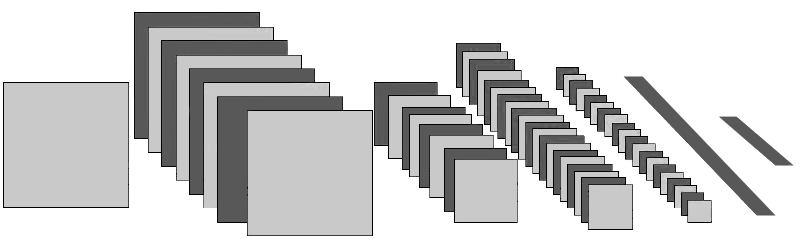
\includegraphics[width=\textwidth]{CNN.png}
	\caption{卷积神经网络\cite{cs231n}}
	\label{CNN}
\end{figure}


卷积神经网络中有三种主要神经层:卷积层、池化层和全连接层\cite{cs231n}。

\subsubsection{卷积层}

如图\ref{3DTensor},我们以RGB三通道图像为例,数字图像在计算机中的表现形式为矩阵排列。RGB图像由三个矩阵叠合而成,每一个矩阵对应一个颜色通道,假设图像的尺寸为$W\times H\times 3$,矩阵中元素的坐标即为相应的像素点,元素的大小代表颜色深度,一个像素点的颜色由三个矩阵中的元素值组合决定。

\begin{figure}[!htp]  
	\begin{minipage}[t]{0.6\linewidth}%设定图片下字的宽度,在此基础尽量满足图片的长宽  
		\centering  
		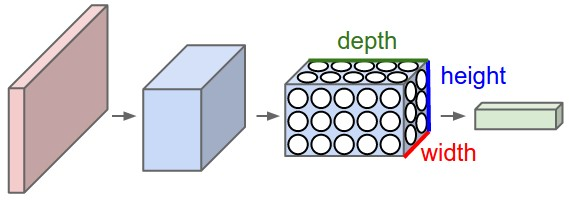
\includegraphics[height=0.13\textheight]{convSizeLeft.jpg}  
		\caption*{(a)}%加*可以去掉默认前缀,作为图片单独的说明  
	\end{minipage}  
	\begin{minipage}[t]{0.4\linewidth}%需要几张添加即可,注意设定合适的linewidth  
		\centering  
		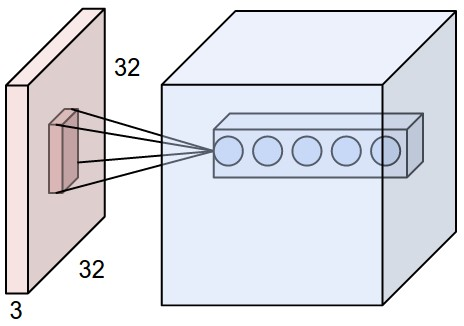
\includegraphics[height=0.13\textheight]{convSizeRight.jpg}  
		\caption*{(b)} 
	\end{minipage}  
	\caption{三维数据表示\cite{cs231n}}%n张图片共享的说明  
	\label{3DTensor}
\end{figure}  


在卷积神经网络中,有一种重要的组件叫做卷积核(又称滤波器),它是一个三维矩阵,长度和宽度需要人为设定,深度必须与输入这一层的数据相等(在这里为3)。卷积核的尺寸远小于图像尺寸,它是卷积层中的共享权重,在计算时需要在数据上平行滑动,被卷积核“套住”的部分与卷积核做内积运算(也即对应位置的元素相乘后再求和)得到一个值,加上偏差后放在新的矩阵的对应位置,接着按照设定的步长在图像上滑动一定距离(此时新矩阵的窗口也向相应位置滑动一格),重复之前的运算,直到遍历整个矩阵。

一个卷积核可以将三维的数据通过上述运算映射成一个二维矩阵,其尺寸由卷积核大小和滑动步长共同决定。有时为了保持卷积运算后矩阵尺寸仍为$W\times H$,我们可以在数据边缘填充数据(其值通常为0),扩展尺寸。

卷积核可以将三维矩阵变换为二维矩阵(也即单通道的三维矩阵),在卷积层中有很多卷积核,其数量通常大于输入数据的通道数。例如,一个有$N$个卷积核的卷积层会把原图像映射成$N$通道的三维矩阵,如果使用零填充维持数据的长和宽,那输出数据的尺寸就为$W\times H\times N$。其运算过程如图\ref{convBlock}所示(这里使用了零填充)。

\begin{figure}[!h]
	\centering
	\animategraphics[width=0.8\textwidth,autoplay,loop,controls]{1}{ConvLayer/ConvLayer_}{0}{17}
	\caption{卷积操作\cite{cs231n}}
	\label{convBlock}
\end{figure}

图\ref{convBlock}是一张动态图,既可以自动播放也能够手动调节。原gif图在源码目录下,如果动画无法正常观看,请自行寻找ConvLayer.gif文件进行观看。

\subsubsection{池化层}

池化层(Pooling Layer)有时也翻译为汇聚层,它的工作是缩小数据尺寸(一般仅缩小长和宽),将相邻的元素合并为一个元素,本质上是对数据的降采样。实现这个功能的组件称为池化层的滤波器。一个2*2的滤波器以2为滑动步长在图像上滑动,可以将图像的长和宽减小到原来的一半,同时,数据也丢失了75\%。

最常用的池化操作为最大池化(Max Pooling),也即在同一通道被滤波器套住的元素中取最大值作为输出。在最大池化之前比较流行的是平均池化(Average Pooling),但实践证明,平均池化效果不如最大池化\cite{cs231n},现在已经很少见了。最大池化操作可以用图\ref{poolingBlock}来表示。

\begin{figure}[!h]
	\centering
	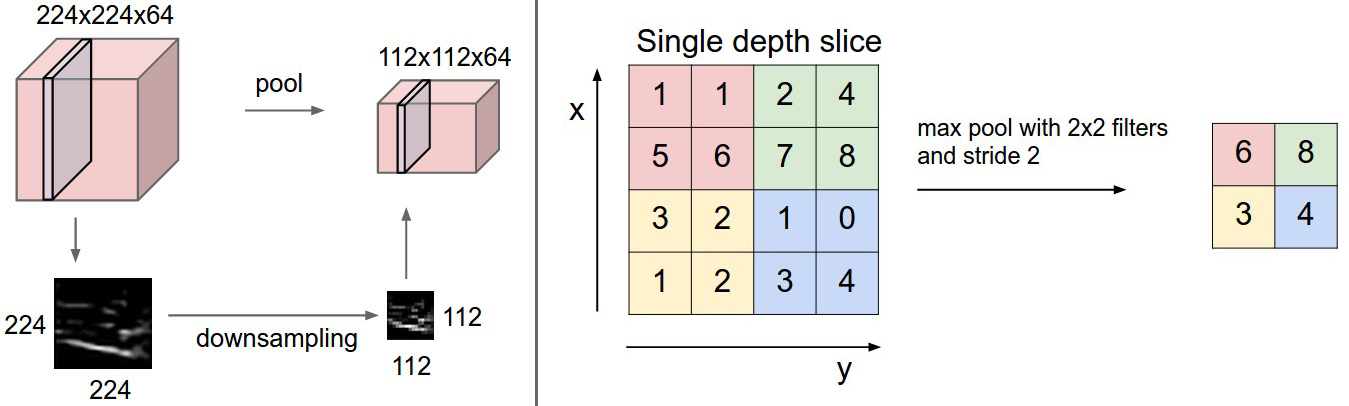
\includegraphics[width=0.8\textwidth]{PoolingLayer.jpg}
	\caption{最大池化操作\cite{cs231n}}
	\label{poolingBlock}
\end{figure}

\subsubsection{全连接层}

在全连接层(Fully Connected Layer)中,神经元对于前一层中的所有激活数据是全部连接的,它们的激活可以先用矩阵乘法,再加上偏差,这和常规神经网络相似,故不再详细阐述。





\section{对神经网络的进一步思考}

\subsection{过拟合与欠拟合}

在训练神经网络的过程中,如果网络的表征能力不够,或者训练方法不当,会导致欠拟合现象,也就是训练出的模型在数据集上没有很好的表现。与此相反的是更易出现的过拟合现象。在训练后期,我们往往会观察到这样的现象:模型在训练集上的精确度逐渐提升,甚至接近完美,但在测试集上的精确度却一成不变,被训练集精确度甩开,有时还会略微下降。究其原因,一是模型对于数据集来说太复杂,二是训练过头。在图\ref{overfitting}中我们能看到,前两个较浅的网络拟合出的函数还具有一定的泛化能力,但第三个深层网络拟合出的函数把太多的数据噪声当成了正常数据,这样的网络无法很好的作出准确预测。

\begin{figure}[!h]
	\centering
	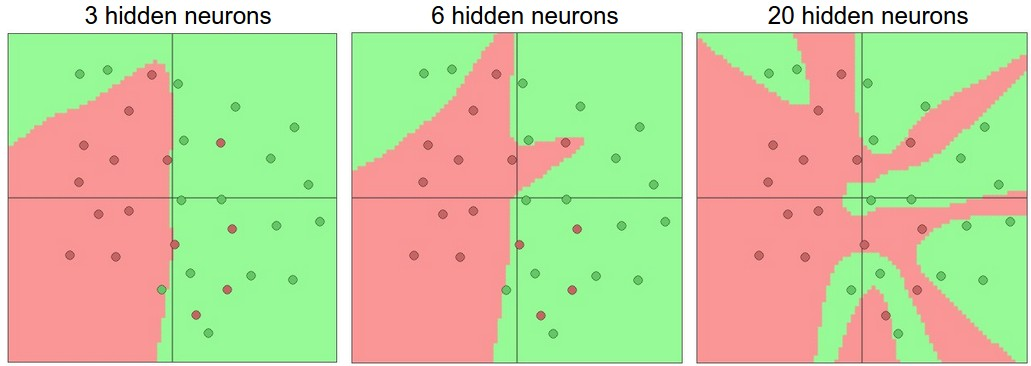
\includegraphics[width=0.8\textwidth]{overfitting.jpg}
	\caption{过拟合现象\cite{cs231n}}
	\label{overfitting}
\end{figure}

缓解过拟合的办法有很多,比较成熟的方法有:1、训练时按一定概率$p$,在隐含层中间屏蔽一些输出,也就是说每个神经元有$p$的概率变为零,不参与前向传播,这种方式称为随机失活(Dropout);2、在损失函数中加入网络中的权重成分,一般对权重平方求和后乘以较小的系数。

\subsection{网络越深,就越好吗?}

在介绍深度学习时我们曾提出一个问题:深度学习的优势在于其网络之深,那我们能不能无限延伸网络结构呢?

答案是否定的。首先,更深的网络会带来更复杂的结构,可能会导致过拟合现象;其次,网络太深会带来庞大的时间和资源消耗,影响整个训练过程;此外,到一定深度之后,仅凭借几种结构的简单重排难以获得进一步提升,要想取得新的突破,必须在网络结构和算法本身加以创新。

\subsection{深度学习只是一种工具}

深度学习对特征的提取很有效,它巧妙的实现了不同特征空间的变换操作,但它不是万能的,只是解决问题的一种工具。要搭出一个好模型,关键还是得根据对任务本身的理解设计合适的算法。不知道要解决什么问题,不去思考怎样抽取数据的特征,盲目套用网络结构,多半是徒劳无功的。

\subsection{多一点耐心}

在深度学习模型的训练中,较为重要的环节除了模型构建和数据读取以外,还要有足够的耐心去调整参数。在整个过程中,任何代码的错误或者不恰当的参数都会使影响训练结果。训练模型本身就是一个循序渐进的过程,一开始可能并不理想,我们需要不断调整学习率等参数,有时甚至需要改造网络结构,重新定义损失函数。心急吃不了热豆腐,所以,多一点耐心。



\section{例题讲解}

\subsection{基于预测公路运量的模型求解}

\subsubsection{问题的提出}

公路运量主要包括公路的客运量和公路货运量两个方面。据研究,某地区的公路运量主要与该地区的人数、机动车数量和公路面积有关,\ref{append}中给出了20年的公路运量相关数据,表中人数和公路客运量的单位为万人,机动车数量单位为万辆,公路面积的单位为万平方千米,公路货运量单位为万吨。

根据有关部门数据,该地区2010年和2011年的人数分别为73.39和75.55万人,机动车数量分别为3.9635和4.0975万辆,公路面积将分别为0.9880和1.0268万平方米。请利用BP神经网络预测该地区2010年2011年得公路客运量和公路货运量。

\subsubsection{BP网络求解过程}

前面已经总结了BP网络求解过程,现在我们通过程序来了解解题的步骤\cite{MATLAB}。

\textbf{原始数据的输入}

\lstset{language=MatLab}
\begin{lstlisting}
clc
%% 原始数据

%人数(单位:万人)
sqrs=[20.55 22.44 25.37 27.13 29.45 30.10 30.96 34.06 36.42 38.09 39.13 39.99 ... 41.93 44.59 47.30 52.89 55.73 56.76 59.17 60.63];
%机动车数(单位:万辆)
sqjdcs=[0.6 0.75 0.85 0.9 1.05 1.35 1.45 1.6 1.7 1.85 2.15 2.2 2.25 2.35 2.5 2.6... 2.7 2.85 2.95 3.1];
%公路面积(单位:万平方公里)
sqglmj=[0.09 0.11 0.11 0.14 0.20 0.23 0.23 0.32 0.32 0.34 0.36 0.36 0.38 0.49 ... 0.56 0.59 0.59 0.67 0.69 0.79];
%公路客运量(单位:万人)
glkyl=[5126 6217 7730 9145 10460 11387 12353 15750 18304 19836 21024 19490 20433 ... 22598 25107 33442 36836 40548 42927 43462];
%公路货运量(单位:万吨)
glhyl=[1237 1379 1385 1399 1663 1714 1834 4322 8132 8936 11099 11203 10524 11115 ... 13320 16762 18673 20724 20803 21804];

%输入数据矩阵
p=[sqrs;sqjdcs;sqglmj]; 
%目标数据矩阵
t=[glkyl;glhyl];         
\end{lstlisting}

\textbf{对输入矩阵和目标矩阵进行归一化}

\lstset{language=MatLab}
\begin{lstlisting}
%% 利用premnmx函数对数据进行归一化
% 对于输入矩阵p和输出矩阵t进行归一化处理
[pn,minp,maxp,tn,mint,maxt]=premnmx(p,t); 
%归一化处理后最小值为-1,最大值为1
dx=[-1,1;-1,1;-1,1];                   
\end{lstlisting}

\textbf{利用处理好的数据对网络进行训练}

\lstset{language=MatLab}
\begin{lstlisting}
%% BP网络训练

%建立模型,并用梯度下降法训练
net=newff(dx,[3,1000,2],{'tansig','tansig','purelin'},'traingdx'); 
%1000次轮回显示一次结果
net.trainParam.show=1000; 
%学习速度为0.05              
net.trainParam.Lr=0.05;    
%最大训练轮回为50000次             
net.trainParam.epochs=50000;    
%均方误差       
net.trainParam.goal=0.65*10^(-3); 
%开始训练,其中pn,tn分别为输入输出样本    
net=train(net,pn,tn);                   
\end{lstlisting}

\textbf{利用训练好的网络对原始数据进行仿真}

\lstset{language=MatLab}
\begin{lstlisting}
%% 利用原始数据对BP网络仿真

%用训练好的模型进行仿真
an=sim(net,pn);   
% 把仿真得到的数据还原为原始的数量级        
a=postmnmx(an,mint,maxt); 
\end{lstlisting}

\textbf{用原始数据仿真的结果与已知的数据进项对比测试}

\lstset{language=MatLab}
\begin{lstlisting}
%% 本例因样本容量有限使用训练数据进行测试
%% 通常必须用新鲜数据进行测试
x=1990:2009;
newk=a(1,:);
newh=a(2,:);
figure (2);
%绘值公路客运量对比图;
subplot(2,1,1);plot(x,newk,'r-o',x,glkyl,'b--+')    
legend('网络输出客运量','实际客运量');
xlabel('年份');ylabel('客运量/万人');
%绘制公路货运量对比图;
subplot(2,1,2);plot(x,newh,'r-o',x,glhyl,'b--+')     
legend('网络输出货运量','实际货运量');
xlabel('年份');ylabel('货运量/万吨');
\end{lstlisting}

\textbf{利用训练好的BP网络对新数据进行仿真}

\lstset{language=MatLab}
\begin{lstlisting}

%% 利用训练好的网络进行预测
%% 当用训练好的网络对新数据pnew进行预测时
%% 也应作相应的处理

%2010年和2011年的相关数据;
pnew=[73.39 75.55
3.9635 4.0975
0.9880 1.0268];   
%利用原始输入数据的归一化参数对新数据进行归一化        
pnewn=tramnmx(pnew,minp,maxp); 
%利用归一化后的数据进行仿真
anewn=sim(net,pnewn);    
%把仿真得到的数据还原为原始的数量级        
anew=postmnmx(anewn,mint,maxt)  ;

\end{lstlisting}

运行这部分程序,我们可以得出2010年和2011年的公路客运量费分别为43790万人和43785万人,公路客运量分别为21704万吨和21705万吨。

网络的学习情况如图\ref{trainResult}所示,可以看出训练的误差很小,达到目标。

\begin{figure}[!h]
	\centering
	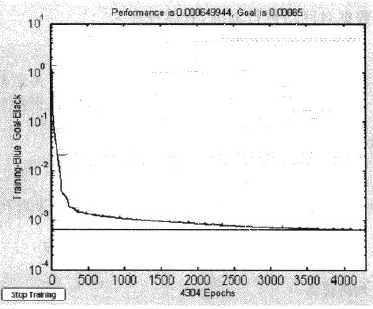
\includegraphics[width=0.6\textwidth]{trainResult.png}
	\caption{网络训练结果}
	\label{trainResult}
\end{figure}

 图\ref{trainResult}是实际样本与网络输出值之间训练和测试的对比图,显然两者之间非常接近,误差极小,因此能够放心进行预测。这里需要说明的是,本案例因为样本数量比较少,测试阶段使用了训练样本。通常情况下,为了测试网络的推理能力,是不宜用训练样本去测试神经网络性能的,应该选用“新鲜”没有使用的数据进行测试。



\subsection{用卷积神经网络进行图像分类}

\subsubsection{问题的提出}

图像分类问题是计算机视觉领域的经典问题,给出一张图片,要求将图片正确归纳到所属类别。ImageNet就是一个可以用于图像分类的庞大数据库,基于ImageNet举办的图像识别竞赛一直是计算机视觉领域的竞争热点。2012年,AlexNet横空出世,大大降低了图像识别的错误率,大家开始意识到卷积神经网络在视觉领域的巨大潜力。

\begin{figure}[!h]
	\centering
	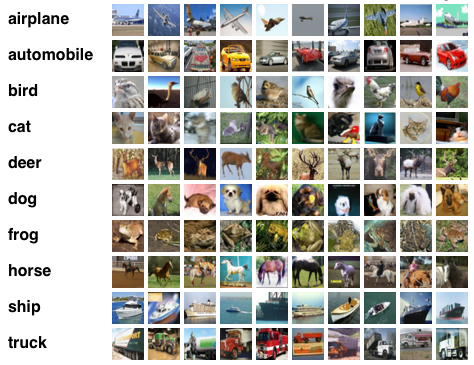
\includegraphics[width=0.7\textwidth]{cifar10.png}
	\caption{CIFAR-10数据集}
	\label{cifar10}
\end{figure}

我们 没有足够的时间和精力去挑战ImageNet,但是可以从简单一些的数据集入手。CIFAR-10是多伦多大学发布的图像数据集\footnote{CIFAR-10下载地址:\url{http://www.cs.toronto.edu/~kriz/cifar.html}},图像总计60000张(其中10000张为测试图像),分为10种,每种6000张,每张图片均为$32\times32\times3$的尺寸\cite{krizhevsky2009cifar}。

与手写数字数据集MNIST\cite{lecun2010mnist}一样,CIFAR-10几乎是入门深度学习和计算机视觉必然接触的数据集。现在请你利用MATLAB搭建一个简单的卷积神经网络,在CIFAR-10上小试身手,训练一个自己的模型。

\subsubsection{模型搭建及训练}

因为涉及卷积神经网络,我们采用了MatConvNet工具箱\footnote{MatConvNet是针对计算机视觉任务开发的神经网络工具箱,包含若干预训练的网络结构,可以完成多种视觉任务,详见\url{http://www.vlfeat.org/matconvnet/}}实现模型。整个任务依旧围绕着构造模型、处理数据和设计训练过程展开,由于代码过长,在此不便展示实现和训练的细节,代码中附有详细注释,数据集可以直接利用给出的代码获取。

因为在Win10系统中并未配置CUDA平台,我们此次利用CPU进行训练,训练速度较慢,我们只进行了40次迭代,top1 error降到了20\%以下,训练结果如图\ref{cifarResult}所示。

\begin{figure}[!h]
	\centering
	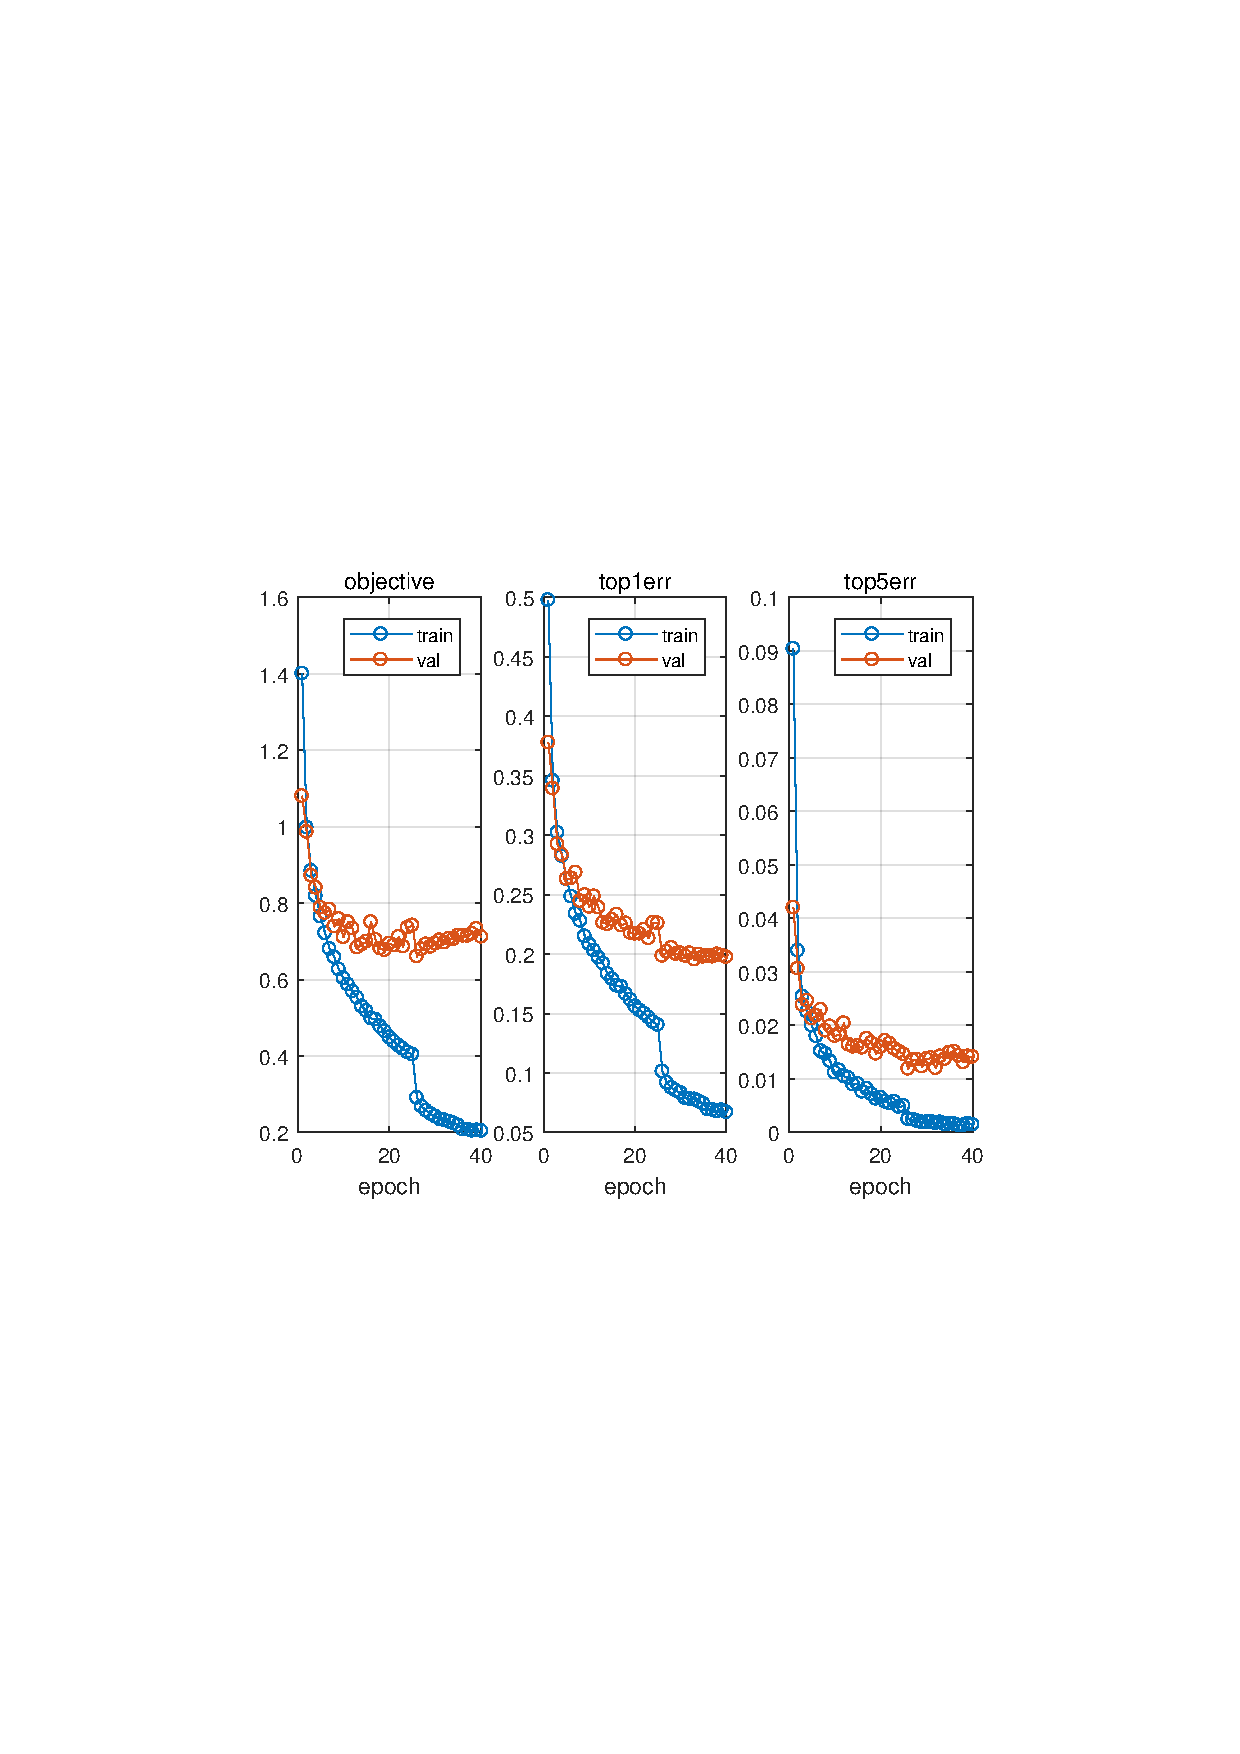
\includegraphics[width=0.8\textwidth]{cifarResult.pdf}
	\caption{CIFAR-10训练结果}
	\label{cifarResult}
\end{figure}

我们将训练的模型用于其他图片上,也取得了不错的结果,如图\ref{cifarDemo}所示。

我们在文件夹中还提供了一份demo代码,文件名为cnn\_cifar\_demo.m,使用方法如下:

\lstset{language=MatLab}
\begin{lstlisting}
>> [Net,Info,Datapre]=cnn_cifar('dataDir','datasetDir');
%不输入参数则会执行默认路径
>> cnn_cifar_demo(Net,'bird.jpg',Datapre);
>> cnn_cifar_demo(Net,'cat.jpg',Datapre);
>> cnn_cifar_demo(Net,'airplane.jpg',Datapre);
\end{lstlisting}

训练开始时代码会优先读取最近保存的模型,如果没有则会创建一个模型。

\begin{figure}[!h] 
	\begin{minipage}[t]{0.5\linewidth}%需要几张添加即可,注意设定合适的linewidth  
		\centering  
		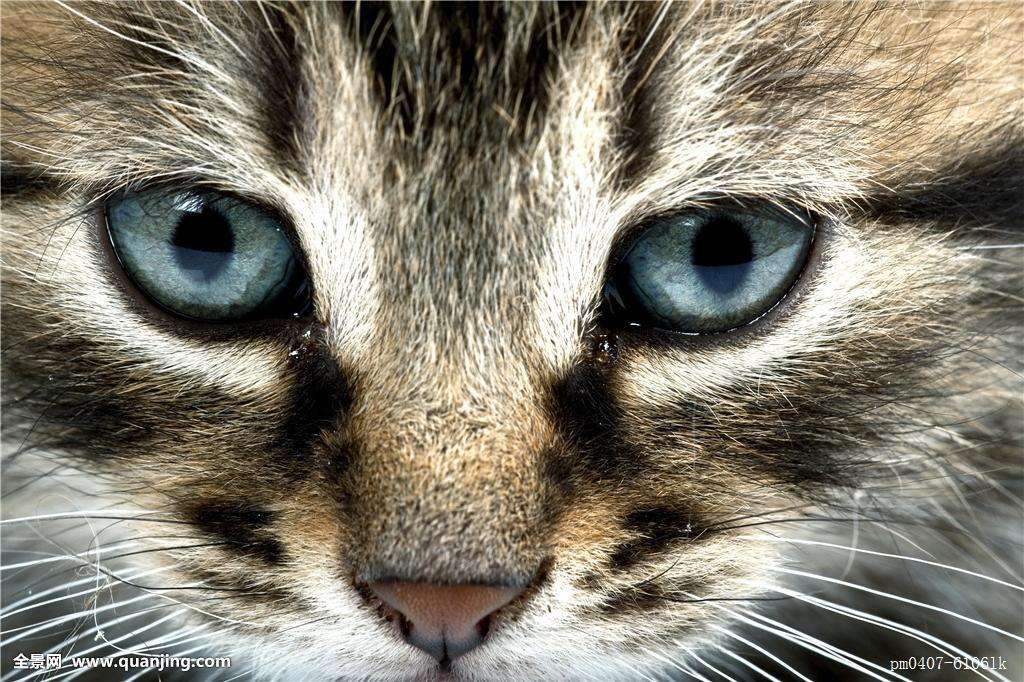
\includegraphics[height=0.29\textheight]{cat.jpg}  
		\caption*{(a)}   
	\end{minipage}  
	\begin{minipage}[t]{0.5\linewidth}%设定图片下字的宽度,在此基础尽量满足图片的长宽  
		\centering  
		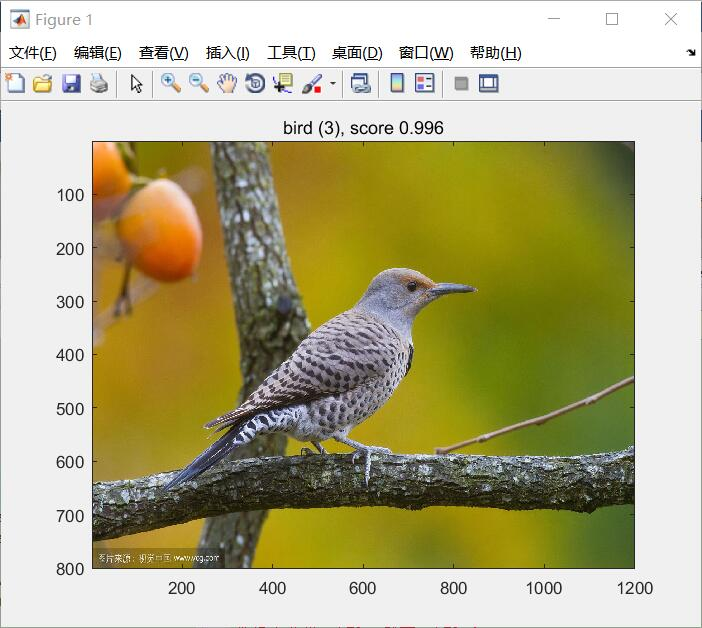
\includegraphics[height=0.29\textheight]{bird.jpg}  
		\caption*{(b)}%加*可以去掉默认前缀,作为图片单独的说明 
	\end{minipage}  
	\caption{训练结果展示}%n张图片共享的说明  
	\label{cifarDemo}
\end{figure} 



\section{神经网络在美赛中的应用}

本部分将介绍神经网络在美赛中的应用,解法分别来自当年的O奖试卷。神经网络在美赛中一般不会作为主干模型,而是被当做解决特定问题的工具,我们先对题目和解法做简要介绍,接下来分析神经网络的应用。详细的题目描述、获奖情况及O奖答卷附在了参考文献目录下。

\subsection{2011 ICM -- C}

\subsubsection{问题的提出}

\begin{shaded}
{
\renewcommand{\baselinestretch}{1.0}

\noindent\textbf{How environmentally and economically sound are electric vehicles?}

\noindent\textbf{Is their widespread use feasible and practical?}

\small\ 

\noindent Here are some issues to consider, but, of course, there are many more, and you will not be able to consider all the issues in your model(s):

\begin{itemize}
\item Would the widespread use of electric vehicles actually save fossil fuels or would we merely be trading one use of fossil fuel for another given that electricity is currently mostly produced by burning fossil fuels? What conditions would need to be put in place to maximize the savings through use of electric vehicles?
\item Consider how much the amount of electricity generated by alternatives such as wind and solar would need to climb during the twenty-first century to make the widespread use of electric vehicles feasible and environmentally beneficial. Assess whether or not the needed growth of these alternate sources of electricity is likely and possible.
\item Would charging batteries at off-peak times be beneficial and increase the feasibility of widespread use of electric vehicles? How quickly would batteries need to charge to maximize the efficiency and practicality of electric vehicles? How would progress in these areas change the equation regarding the environmental savings and practicality of widespread use of electric vehicles?
\item What method of basic transportation is most efficient? Is the efficiency of different methods dependent of the nation or region in which it is used?
\item Pollution caused directly by electric vehicles is low, but are there hidden sources of pollutants associated with electric vehicles? Gasoline and diesel fuel burned in internal combustion engines for transportation account for nitrites of oxygen, vehicle-born monoxide and carbon dioxide pollution but are these bi-products something we really should worry about? What are the short and long term effects of these substances on the climate and our health?
\item How would the pollution caused by the increasing need to dispose of increasing numbers of large batteries effect the comparison between the environmental effects of electric vehicles versus the effects of fossil fuel-burning vehicles?
\item You also should consider economic and human issues such as the convenience of electric vehicles. Can batteries be recharged or replaced fast enough to meet most transportation needs or would their ranges be limited? Would electric vehicles have only a limited role in transportation, good only for short hauls (commuters or light vehicles on short trips) or could they practically be used for heavier and longer-range transportation and shipping? Should governments give subsidies to developers of electric vehicle technologies and if so, why, how much, and in what form?
\end{itemize}

\noindent\textbf{Requirements:}
\begin{itemize}
\item Model the environmental, social, economic, and health impacts of the widespread use of electric vehicles and detail the key factors that governments and vehicle manufacturers should consider when determining if and how to support the development and use of electric vehicles. What data do you have to validate your model(s)?
\item Use your model(s) to estimate how much oil (fossil fuels) the world would save by widely using electric vehicles.
\item Provide a model of the amount and type of electricity generation that would be needed to support your recommendations regarding the amount and type of electric vehicle use that will produce the largest number of benefits to the environment, society, business, and individuals.
\item Write a 20-page report (not including the summary sheet) to present your model and your analysis of the key issues associated with the electric vehicle and electricity generation. Be sure to include the roles that governments should play to insure safe, efficient, effective transportation. Discuss if the introduction of widespread use of electric vehicles is a worthwhile endeavor and an important part of an overall strategy to address global energy needs in the face of dwindling fossil fuel supplies.

\end{itemize}

\noindent\rule{\textwidth}{0.1mm}
\normalsize\ 

\noindent\textbf{电动汽车的环保性和经济性如何?}

\noindent\textbf{它们的广泛使用是否可行和实际?}

\small\ 

\noindent 这里有一些问题需要考虑,当然不止这些,你不必在自己的模型中涵盖所有问题:

\begin{itemize}
\item 电动汽车的广泛使用是否真的能节省化石燃料,还是说我们是在用另一种燃料交换化石燃料(因为当下的电力主要通过消耗燃料产生)?需要什么条件来最大程度上节省电动汽车的费用?
\item 考虑诸如风能和太阳能等替代能源需要产生多少电力,才能使普及电动汽车成为实际可行且有益环境的选择?请评估是否应该增加替代能源来产生电力。
\item 在非高峰时段使用充电电池会有助于提升电动汽车广泛使用的可行性吗?电池充电速度多快才能使汽车的效率和可行性最大化?这些领域的进展会如何改变节约环境资源和普及电动汽车之间的关系?
\item 怎样的基本交通方式最有效率?各种方法的效率是否依赖于使用的国家或地区?
\item 电动汽车产生的直接污染很小,但是否存在与电动汽车有关的间接污染源?交通运输中内燃机燃烧汽油和柴油会产生含亚硝酸盐的氧气、一氧化碳和二氧化碳,但我们担心的真的是这些副产品吗?这些物质对气候和我们的健康有什么短期和长期影响?
\item 处理日益增多的电池会带来污染,它将如何影响电动汽车和燃料汽车对环境影响的比较?
\item 你还应考虑经济和人方面的问题,比如电动汽车的便利性。电池充电或替换的速度能满足大多数交通需求吗,还是说它们的范围受到限制?电动汽车在交通运输中是作用有限、仅对小型运输(轻型车辆或短途运输)有帮助,还是对大型长途运输也有实际帮助?政府是否应该向电动汽车技术的开发人员提供补贴?如果需要的话,请阐述补贴原因、补贴程度及补贴形式。
\end{itemize}

\noindent\textbf{要求:}

\begin{itemize}
\item 针对电动汽车的普及带来的环境、社会、经济和健康影响建立模型,详细陈述政府和汽车厂商在决定是否及如何推广电动汽车时应当考虑的关键因素。你的模型需要什么样的数据加以验证?
\item 用你的模型估计全球普及电动汽车后能节省多少石油(化石燃料)。
\item 请提供一个关于发电类型及产量的模型,以支撑你对电动汽车类型和数量的建议,给环境、社会、商业及个体带来最大程度的利益。
\item 撰写一份20页的报告(不包括摘要页),展示你的模型,分析电动汽车和电力生产中的关键问题。为确保安全、高效和有效的运输,报告中要包括政府应该扮演的角色。讨论电动汽车的推广是否是一项有价值的尝试,是否是在化石能源日益减少时应对全球能源需求的总体战略的重要组成部分。
\end{itemize}

}

\end{shaded}

\subsubsection{解题思路}

本题解答来自2011年ICM的9089号队伍。

本模型讨论了以下问题:(1)分析普及电动汽车的环境、经济、健康和社会影响;(2)确定待考虑的关键因素,以决定是否及如何推广电动汽车;(3)预测在推广电动汽车后全世界节省的化石燃料有多少;(4)优化能源网络以适应电动汽车的广泛使用,使得环境、社会、商业和个体都能获得最大程度的利益。

针对上述问题建立模型,用到的主要方法有:(1)运用基于蚁群优化算法的贝叶斯模型预测电动汽车的销售情况;(2)用灰度模型改进BP神经网络并预测未来十年世界汽车总量,计算排放量减少值;(3)建立多目标规划模型优化现有的能源结构,探索用清洁能源生产电力的最佳比例,并用层次分析法简化模型。

对于汽车总量的预测问题,首先想到的方法是灰度模型(GM)。令$E(i)$表示第$i$年汽车的总量,规定$E_0$是关于$E(i)$的一个序列
\[E_0 = (E(1),E(2),\cdots),E(n)\]
$E_1$是关于$E_0$的顺序累加序列,即
\[E_1 = (E_1(1),E_1(2),\cdots,E_1(n))\]
其中$E_1(k) = \Sigma_{i=1}^kE_0(i),k=1,2,\cdots,n$。

令$Z$表示序列
\[
\begin{split}
Z &= (z(2),z(3),\cdots,z(k))\\
z(k) &= \frac{1}{2} (E_1(k)+E_1(k-1))
\end{split}
\]

在此基础上,令$Y=\left[
\begin{matrix}
E(2)\\
E(3)\\
\vdots\\
E(n)
\end{matrix}\right]
$,$B=\left[
\begin{matrix}
-z(2) & 1\\
-z(3) & 1\\
\vdots & \vdots\\
-z(n) & 1
\end{matrix}\right]
$,通过对等式$E(k)+az(k)=b$的最小二乘估计,我们有
\[[a,b]^T = (B^T B)^{-1} B^T Y\]

最终能得出
\[\hat{E_1}(k+1) = (E(1)-\frac{b}{a})\mathrm{e} ^{-ak} + \frac{b}{a}, k=1,2,\cdots,n\]
\[\hat{E}(k) = \hat{E_1}(k) - \hat{E_1}(k-1)\]

但在这一问中GM并没有被直接用来解决预测问题,最主要的原因是GM虽然能很好的预测数据的变化趋势,但难以做出复杂的非线性拟合。因此考虑将GM与BP神经网络结合起来对汽车总量进行预测。保留GM中的累加运算和累减运算,用神经网络做参数拟合,以得到最终的预测结果。

\subsection{2013 MCM -- A}

\subsubsection{问题的提出}

\begin{shaded}
\renewcommand{\baselinestretch}{1.0}
\begin{center}
\textbf{The Ultimate Brownie Pan}
\end{center}

\small\noindent
When baking in a rectangular pan heat is concentrated in the 4 corners and the product gets overcooked at the corners (and to a lesser extent at the edges). In a round pan the heat is distributed evenly over the entire outer edge and the product is not overcooked at the edges. However, since most ovens are rectangular in shape using round pans is not efficient with respect to using the space in an oven. Develop a model to show the distribution of heat across the outer edge of a pan for pans of different shapes - rectangular to circular and other shapes in between.\newline

\noindent Assume
\begin{enumerate}
\item A width to length ratio of W/L for the oven which is rectangular in shape.
\item Each pan must have an area of A.
\item Initially two racks in the oven, evenly spaced.
\end{enumerate}\ 

\noindent Develop a model that can be used to select the best type of pan (shape) under the following conditions:
\begin{enumerate}
\item Maximize number of pans that can fit in the oven (N)
\item Maximize even distribution of heat (H) for the pan
\item Optimize a combination of conditions (1) and (2) where weights p and (1- p) are assigned to illustrate how the results vary with different values of W/L and p.
\end{enumerate}\ 

\noindent In addition to your MCM formatted solution, prepare a one to two page advertising sheet for the new Brownie Gourmet Magazine highlighting your design and results.

\noindent\rule{\textwidth}{0.1mm}
\normalsize\ 
\begin{center}
\textbf{终极巧克力蛋糕锅}
\end{center}

\small\noindent 
当在一个矩形锅中烘烤时,热量集中在四个角落,产品在角落处会烤过头(边缘的较小范围内)。
在一个圆形的锅中热量被均匀地分布在整个外缘使得在边缘的食物不会烘烤过度。然而,由于大
多数烤箱是长方形的,圆形的锅空间利用率不高。请建立一个模型来显示热量在不同形状的锅的
外缘的分布情况——锅的形状是从矩形过渡到圆形的各种形状。\newline

\noindent 假设
\begin{enumerate}
\item 矩形烤箱的宽长比是W/L。
\item 每个锅的面积是A。
\item 最开始,烤箱中均匀放置由两个锅。
\end{enumerate}\ 

\noindent 请建立一个模型,在满足以下条件下可得到锅的最佳形状。
\begin{enumerate}
\item 最大化烤箱中锅的数量(N)
\item 最大限度地平衡锅的热量分布(H)
\item 最优化条件(1)和(2)的组合,并引入条件(1)和(2)的权重p和(1-p)来描述结果如何随W/L和p的值变化。
\end{enumerate}\ 

\noindent 除了MCM的格式化的解答,为巧克力蛋糕美食杂志准备一至两页的广告来突出你的设计和成果。
\end{shaded}

\subsubsection{解题思路}

本题解答来自2013年MCM的20329号队伍。

该题我们需要建立两个模型。一个是热量分布模型,一个是锅的形状模型。其中锅的形状是分析一切的基础。
文章以三个参数长、宽、圆角半径定义了一个圆角矩形模型,并进一步在此基础上展开了热量分布的分析。
在热量分布的分析过程中,文章通过构造带有边界约束条件的二维热平衡方程来解题。对于圆形和矩形,给出了
固定的解法,对于中间形状的圆角矩形,采用有限元法(FEM)给出数值解。最终发现锅内的温度分布是均匀的,而
锅的形状的对于边缘的分布影响较大。因此,文中定义了一个衡量边缘分布均匀程度的参数$\mu$,并采用神经网络来对
$\mu$进行拟合。

关于题中的第二个任务,在此前的基础上能够较为轻松地得到矩形与圆形分别是条件(1)和条件(2)的最优解。在条件
(3)中,通过p的变化,将得到不同形状的圆角矩形,宽高比W/L对形状的影响相对较明显。

下面对其中使用神经网络的详细介绍。文中使用的是一个两层的反馈神经网络,由Matlab的神经网络工具箱进行实现,
一个隐层的激活函数采用了sigmoid函数,输出为线性输出。网络以$(w,l)$作为输入,以$\mu$作为输出,因此需
要一个二元输入层神经元,一个输出层神经元。图\ref{2013ann}展示了该网络的结构图示,该图示由Matlab神经网络工具箱自动绘制。
网络模型中的其它参数均由Matlab神经网络工具箱默认设置。

\begin{figure}[!h]
	\centering
	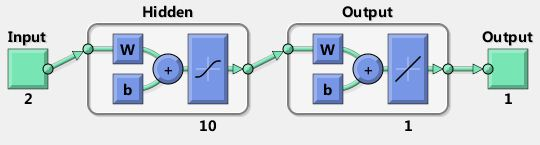
\includegraphics[width=0.8\textwidth]{2013ANN.jpg}
	\caption{神经网络结构图示}
	\label{2013ann}
\end{figure}

具体操作时,首先需要预计算一定量的数据后,即采用文中方法所计算的部分$w,l$即相应的$\mu$
值。再利用这些数据对该网络进行训练,使得网络逐渐接近真实的函数模型。经过一定程度的训练后,最终得到的
网络模型类似于一个有较好拟合度的以$w,l$为自变量,$\mu$为因变量的二元非线性函数。具体的函数接口可参
考Matlab神经网络工具箱的帮助文档。

\subsection{2013 MCM -- B}

\subsubsection{问题的提出}

\begin{shaded}
\renewcommand{\baselinestretch}{1.0}
\begin{center}
\textbf{Water, Water, Everywhere}
\end{center}

\small\noindent
Fresh water is the limiting constraint for development in much of the world. Build a mathematical model for determining an effective, feasible, and cost-efficient water strategy for 2013 to meet the projected water needs of [pick one country from the list below] in 2025, and identify the best water strategy. In particular, your mathematical model must address storage and movement; de-salinization; and conservation. If possible, use your model to discuss the economic, physical, and environmental implications of your strategy. Provide a non-technical position paper to governmental leadership outlining your approach, its feasibility and costs, and why it is the “best water strategy choice.”
\newline

\noindent Countries: United States, China, Russia, Egypt, or Saudi Arabia

\noindent\rule{\textwidth}{0.1mm}
\normalsize\ 
\begin{center}
\textbf{水,水,无处不在}
\end{center}

\small\noindent 
淡水是世界大部分地区发展的制约因素。建立一个数学模型来为2013年确定一个有效、可行并且成本效益高的水资源策略,以满足2025年[下列国家中选择一个国家]的预计用水需求,并且确定最佳的水资源策略。尤其重要的是,你的数学模型需要解决存储和移动、去盐碱化以及保护的问题。如果可能,请用你的模型来讨论你的策略对经济、物理以及环境造成的影响。向政府领导提供一份非技术的立场文件来概述你的方法、可行性和成本,以及为什么这是“水资源策略的最佳选项”。\newline

\noindent 国家:美国、中国、俄罗斯、埃及、沙特阿拉伯
\end{shaded}

\subsubsection{解题思路}

本题解答来自2013年MCM的21185号队伍。

对于我国(中国),我们目前遇到的水资源问题主要为三类:北部和西北部水资源匮乏;南方地区洪涝灾害严重;工业和农业生产造成的污水太多。

为了满足题目的要求,我们可以将问题划分为五个子问题:
\begin{enumerate}
\item 基于历史数据对未来13年(2013-2025)的用水量需求进行预测。
\item 建立全国水资源存储和移动策略的模型以解决中国水资源时间空间上分布不均的问题。
\item 设计区域水资源去盐碱化策略的模型来增加可用水资源总量。
\item 建立水资源保护策略的模型,包括区域水污染的处理和全国节水策略。
\item 上述四种水利方案的长期成本效益分析和水利方案最优组合的讨论。
\end{enumerate}

对于第一个子问题,文中采用了灰色Verhulst模型进行了很好的处理,较好地对2013-2025年的用水量需求进行了预测。对于第二个子问题,采用了目标规划建立了存储的模型,利用最小生成树算法提出了最佳的水资源传输方案。第三个子问题及第四个子问题文中都根据实际情况定义了一定的参数,并在此基础上进一步建立了相关的数学模型。最后的第五个子问题上,文章首先用层次分析法分析了经济,物理和环境影响的权重。 然后用神经网络算法对各个策略的质量进行分类,最后得到一个合理的策略评估模型。下面对神经网络的具体应用进行详细介绍。

其中神经网络的输入为$m_i=(ec_i,ph_i,en_i,others_i)$,其中$ec_i$,$ph_i$,$en_i$均为由层次分析法得到的影响级别(经济、物理、环境),
$others_i$仅为表示属性能够扩展的标志。输出则为一个1到10的质量级别。利用神经网络对策略质量进行分类的具体步骤如下:
\begin{enumerate}
\item 首先收集影响级别和质量级别的数据,对神经网络进行训练。
\item 然后对于每个水资源策略由层次分析法得到$m_i$中的属性。
\item 将$m_i$输入到预训练好的神经网络模型中。
\item 分析输出的质量等级结果。
\end{enumerate}

\subsection{2016 ICM -- D}

\subsubsection{问题的提出}

\begin{shaded}
{\setlength\parindent{1em}
\renewcommand{\baselinestretch}{1.0}
\begin{center}
\textbf{Measuring the Evolution and Influence in Society's Information Networks}
\end{center}

\small
\noindent Information is spread quickly in today's tech-connected communications network; sometimes it is due to the inherent value of the information itself, and other times it is due to the information finding its way to influential or central network nodes that accelerate its spread through social media. While content has varied -- in the 1800s, news was more about local events (e.g., weddings, storms, deaths) rather than viral videos of cats or social lives of entertainers -- the prevailing premise is that this cultural characteristic to share information (both serious and trivial) has always been there. However, the flow of information has never been as easy or wide-ranging as it is today, allowing news of various levels of importance to spread quickly across the globe in our tech connected world. By taking a historical perspective of flow of information relative to inherent value of information, the Institute of Communication Media (ICM) seeks to understand the evolution of the methodology, purpose, and functionality of society's networks.\newline

\noindent Specifically, your team, as part of ICM's Information Analytics Division, has been assigned to analyze the relationship between speed/flow of information vs inherent value of information based on consideration of 5 periods: in the 1870s, when newspapers were delivered by trains and stories were passed by telegraph; in the 1920s, when radios became a more common household item; in the 1970s, when televisions were in most homes; in the 1990s, when households began connecting to the early internet; in the 2010s, when we can carry a connection to the world on our phones. Your supervisor reminds you to be sure to report the assumptions you make and the data you use to build your models.\newline

\noindent Your specific tasks are:
\begin{enumerate}
\item Develop one or more model(s) that allow(s) you to explore the flow of information and filter or find what qualifies as news.
\item Validate your model's reliability by using data from the past and the prediction capability of your model to predict the information communication situation for today and compare that with today's reality.
\item Use your model to predict the communication networks' relationships and capacities around the year 2050.
\item Use the theories and concepts of information influence on networks to model how public interest and opinion can be changed through information networks in today's connected world.
\item Determine how information value, people's initial opinion and bias, form of the message or its source, and the topology or strength of the information network in a region, country, or worldwide could be used to spread information and influence public opinion.
\end{enumerate}


\noindent\rule{\textwidth}{0.1mm}
\normalsize\ 
\begin{center}
\textbf{社会信息网络中的演变和影响评估}
\end{center}

\small\ 

\noindent 信息在当今由技术连接的通信网络中得到迅速传播;有时是因为信息本身的内在价值,有时是因为信息找到有影响力的中心网络结点,通过社交媒体加速传播。尽管内容有所不同——在19世纪,新闻关注的更多是当地的事件(如婚礼、风暴、死亡等)而不是猫的热点视频或艺人的社交生活——最普遍的前提是,这种分享信息(不论是严肃的还是琐碎的)的文化特征一直存在。然而,信息的流动从来没有像今天这样简单和广泛,允许不同重要程度的新闻通过互联网世界迅速传遍全球。通过对信息流相对于信息内在价值的历史透视,传播媒体研究所(ICM)试图去理解社会网络方法、目的和功能的演变。\newline

\noindent 具体来说,作为ICM信息分析部门的一部分,你们团队被分配去分析信息流动(速度)与信息内在价值的关系,分为以下五个时间段:19世纪70年代,报纸通过火车发行,事件通过电报传递;20世纪20年代,收音机成为常见的家用物品;20世纪70年代,大多数家庭拥有了电视;在20世纪90年代,家庭互联网初具雏形;2010年左右,我们使用手机与世界相连。部门主管请你们切记在报告中阐明你们的假设及建模时用到的数据。\newline

\noindent 你们的具体任务如下:
\begin{enumerate}
\item 设计一个或多个模型,探索信息的流动,过滤或找出什么才能作为新闻。
\item 用过去的数据和模型的预测能力预测现在的信息通信情况并与实际情况相比较,以此验证模型的可靠性。
\item 用你的模型去预测2050年前后通信网络的关系和容量。
\item 运用信息影响网络的理论的和概念进行建模,分析当今的互联世界中公众热点和舆论如何通过信息网络被改变。
\item 确定信息价值、人们的初始意见及偏差、信息形式或来源、区域(或国家、全球)的信息网络结构或强度是如何被用来传播信息、影响公众舆论的。
\end{enumerate}
}

\end{shaded}

\subsubsection{解题思路}
本题解答来自2016年ICM的47876号队伍。

整个模型分为四部分:

\textbf{Information Circulation Network Model(ICN)}\quad 针对不同年代构造了五种不同的网络拓扑结构,量化分析年代变迁中信息网络的演化。

\textbf{News Filter Model(NF)}\quad 一种模糊综合评价模型,提出了信息价值的评价指标——audience awareness index (AAI),并用此判断某条信息是否为新闻。

\textbf{Information Circulation Network Prediction Model(ICNP)}\quad 一种BP神经网络预测模型,预测信息网络的关系和容量。

\textbf{Public Interest and Information Network Interaction Model(PIINI)}\quad 在考虑信息循环网络和公众兴趣交互的基础上,建立了兴趣衰减机制和社交强化机制。

其中ICNP模型运用了BP神经网络预测信息网络的关系和容量,下面进行介绍。

\textbf{输入输出定义}\quad 根据题目要求和ICN模型的定义,在ICNP模型中将网络输出定义为信息循环网络的结点数量和度数。基于现实情况,将网络输入量定义为三个指标:区域经济水平(GDP)、区域通信水平(IDI\footnote{维基百科:\url{https://en.wikipedia.org/wiki/ICT_Development_Index}})、区域教育水平(EI\footnote{维基百科:\url{https://en.wikipedia.org/wiki/Education_Index}})。

\textbf{数据预处理}\quad 数据来源于美国三个州的互联网:California(CA)、Texas(TX)和New York(NY)。数据的归一化采用如下公式:
\[\hat{X_i} = \frac{X_i - X_{\min}}{X_{\max} - X_{\min}}\]

\textbf{模型验证}\quad 在验证集上将ICN和ICNP的结点数量及度数进行对比,结果见表\ref{tbl:2016d1}。

\begin{table}[!h]
\begin{center}
\caption{During the sample period prediction}
\label{tbl:2016d1}
\renewcommand{\arraystretch}{0.5}
\begin{tabular}{c|ccc}
\hline
& From ICN model & From predict model & Relative error (\%)\\ \hline
Number of node (person) & 19541453 & 22535000 & 15.32\\
Degree of node (person) & 11223538 & 13533000 & 20.58\\ \hline
\end{tabular}
\end{center}
\end{table}

\textbf{预测结果}\quad 将训练好的模型用于预测2050年信息网络的关系和容量,结果见表\ref{tbl:2016d2}。

\begin{table}[!h]
\begin{center}
\caption{During the sample period prediction}
\label{tbl:2016d2}
\begin{tabular}{c|c}
\hline
& From ICNP model\\ \hline
Number of node (person) & 34885000\\
Degree of node (person) & 23766000\\ \hline
\end{tabular}
\end{center}
\end{table}

\newpage
\bibliographystyle{unsrt}
\bibliography{ref.bib}

\appendix
\section{例题一所需数据}
\label{append}
\begin{table}[H]
	\centering
	\label{tbl:data}
	\caption{某地区20年公路运量数据}
	\begin{tabular}{|c|c|c|c|c|c|}
		\hline		
		年份 & 人口数量/万人 & 公路面积/万平方千米 & 公路客运量/万人& 累计 & 公路货运量/万吨\\ \hline
		1990 & 20.55 & 0.6 & 0.09 & 5126 & 1237\\ \hline
		1991  & 22.44  & 0.75 &  0.11 &  6217  & 1379\\ \hline
		1992 &  25.37  & 0.85 &  0.11 &  7730 &  1385\\ \hline
		1993 &  27.13 &  0.90 &  0.14 &  9145 &  1399\\ \hline
		1994 &  29.45 &  1.05 &  0.20 &  10460 &  1663\\ \hline
		1995 &  30.1  & 1.35 &  0.23  & 11387 &  1714\\ \hline
		1996 &  30.96 &  1.45 &  0.23 &  12353 &  1834\\ \hline
		1997  & 34.06 &  1.60 &  0.32 &  15750 &  4322\\ \hline
		1998  & 36.42 &  1.70 &  0.32 & 18304 &  8132\\ \hline
		1999  & 38.09 &  1.85 &  0.34 &  19836 &  8936\\ \hline
		2000 &  39.13 &  2.15 &  0.36 &  21024 &  11099\\ \hline
		2001  & 39.99 &  2.20 &  0.36 &  19490 &  11203\\ \hline
		2002 &  41.93 &  2.25 &  0.38 &  20433 &  10524\\ \hline
		2003 &  44.59 &  2.35 &  0.49 &  22598 &  11115\\ \hline
		2004  & 47.30 &  2.50 &  0.56 &  25107 &  13320\\ \hline
		2005  & 52.89 &  2.60 &  0.59 &  33442  & 16762\\ \hline
		2006 &  55.73 &  2.70 &  0.59 &  36836 & 18673\\ \hline
		2007  & 56.76 &  2.85 &  0.67 &  40548 &  20724\\ \hline
		2008  & 59.17 &  2.95 &  0.69 &  42927 &  20803\\ \hline
		2009 &  60.63 &  3.10 &  0.79 &  43462  & 21804\\ \hline	
	\end{tabular}
\end{table}


\end{document} 